\documentclass[12pt,italian,a4paper,oneside,openright]{book}
\usepackage{url,amsfonts,epsfig}
\usepackage[italian]{babel}
\usepackage[T1]{fontenc}
\usepackage[utf8]{inputenc}
\usepackage{lmodern}
\usepackage{vmargin}
\usepackage{amsmath}
\usepackage{indentfirst}
\usepackage{graphicx}
\usepackage{listings}
\usepackage{xcolor}
\graphicspath{{img/}}
\usepackage[hyperindex]{hyperref}
\hypersetup{colorlinks=true, linkcolor=black}
\sloppy

\setmarginsrb{35mm}{30mm}{30mm}{30mm}{0mm}{10mm}{0mm}{10mm}

\usepackage{fancyhdr}
\setlength{\headheight}{15pt}
\addtolength{\topmargin}{-3pt}
\pagestyle{fancy}
\fancyhf{}
\fancyhead[C]{\leftmark}
\fancyfoot[C]{\thepage}
\renewcommand{\headrulewidth}{0.4pt}
\DeclareGraphicsRule{.jpg}{jpg}{}{}

% Stile per listati C++
\lstset{
    language=C++,
    basicstyle=\ttfamily\small,
    keywordstyle=\color{blue}\bfseries,
    commentstyle=\color{gray}\itshape,
    stringstyle=\color{orange},
    numberstyle=\tiny\color{gray},
    numbers=left,
    stepnumber=1,
    frame=single,
    breaklines=true,
    captionpos=b,
    tabsize=4
}

\title{Relazione ASD --- Traccia 1: HashRBTree}
\author{Raffaele Calcagno}
\date{A.A. 2021--2022}

\begin{document}
\pagenumbering{Roman}
\baselineskip 1.5em

%% FRONTESPIZIO
{\thispagestyle{empty}
\vskip 1cm \large \centerline{\textsc{Universit\'a degli Studi di
Napoli ``Parthenope''}}
\centerline{\textsc{Scuola interdipartimentale delle Scienze, dell'Ingegneria e della Salute}}
\centerline{\textsc{Dipartimento di Scienze e Tecnologie}}
\centerline{\small\textsc{Corso di laurea in Informatica}}
\begin{center}

\includegraphics[scale=0.24]{images/logo.png}
\end{center}
\vskip 0.5cm
\large \centerline{\textsc{Relazione di Algoritmi e Strutture Dati}}
\vskip 0.5cm
\Large \centerline{Traccia 1 --- Esercizio 1}
\Large \centerline{HashRBTree}
\vskip 4.5cm
\large
\begin{minipage}[t]{7cm}
\textsc{Docente}\\
Prof. Ferone\\
\end{minipage}
\hfill
\begin{minipage}[t]{5cm}
\textsc{Studente}\\
Raffaele Calcagno\\
0124001717
\end{minipage}
\vskip 2.0cm \Large \centerline{Anno Accademico 2021--2022}
\vfill \eject}

\pagenumbering{arabic}
\chapter{Descrizione del Problema}

Il problema richiede la progettazione e l'implementazione di una struttura dati ibrida 
denominata \textbf{HashRBTree}, che combina le proprietà di una funzione di hash con 
quelle di un albero Red-Black (RBT).

L'obiettivo è realizzare una struttura in grado di memorizzare coppie 
\texttt{(chiave, valore)} di tipo stringa, supportando efficientemente le operazioni 
fondamentali di un dizionario:

\begin{itemize}
    \item \textbf{Inserimento} di una coppia \texttt{(chiave, valore)};
    \item \textbf{Ricerca} del valore associato a una chiave;
    \item \textbf{Cancellazione} di una coppia \texttt{(chiave, valore)}.
\end{itemize}

\section{Approccio Adottato}

La chiave viene trasformata in un intero tramite una funzione di hash, che diventa 
l'identificatore (\texttt{id}) del nodo all'interno dell'albero Red-Black. 
L'albero è quindi organizzato sui valori di \texttt{id}, garantendo ricerca, 
inserimento e cancellazione in tempo $O(\log n)$.

Le \textbf{collisioni} --- situazioni in cui due chiavi diverse producono lo stesso 
valore di hash --- vengono gestite tramite una lista concatenata associata a ciascun 
nodo. Ogni nodo dell'albero mantiene una \texttt{std::list} di coppie 
\texttt{(chiave, valore)}, consentendo la coesistenza di più entry con lo stesso 
identificatore.

\section{Motivazioni della Scelta}

La combinazione di hash e Red-Black Tree offre un compromesso vantaggioso:

\begin{itemize}
    \item La \textbf{funzione di hash} riduce lo spazio delle chiavi (stringhe 
    arbitrarie) a un insieme di interi, rendendo possibile un ordinamento totale 
    dei nodi;
    \item Il \textbf{Red-Black Tree} garantisce il bilanciamento automatico 
    dell'albero, assicurando complessità logaritmica nel caso peggiore a differenza 
    delle hash table classiche che degradano a $O(n)$ in caso di molte collisioni;
    \item La \textbf{lista di collisione} per nodo gestisce in modo semplice ed 
    efficace le rare collisioni di hash senza richiedere strutture aggiuntive.
\end{itemize}
\chapter{Descrizione delle Strutture Dati}

\section{KeyValue}

La struttura \texttt{KeyValue} rappresenta la coppia chiave-valore memorizzata 
nella lista di collisione di ciascun nodo. È definita come segue:

\begin{lstlisting}
struct KeyValue {
    string key;
    string value;
};
\end{lstlisting}

Entrambi i campi sono di tipo \texttt{std::string}. La separazione della coppia 
in una struttura dedicata rende il codice più leggibile e facilita la gestione 
delle collisioni nella lista.

\section{RBNode}

\texttt{RBNode} rappresenta il nodo dell'albero Red-Black. Ogni nodo contiene:

\begin{itemize}
    \item \texttt{int id} --- identificatore numerico del nodo, ottenuto applicando 
    la funzione di hash alla chiave inserita;
    \item \texttt{Color color} --- colore del nodo, \texttt{RED} o \texttt{BLACK}, 
    necessario per mantenere le proprietà dell'albero Red-Black;
    \item \texttt{std::list<KeyValue> items} --- lista concatenata delle coppie 
    \texttt{(chiave, valore)} che condividono lo stesso valore di hash (gestione 
    delle collisioni);
    \item \texttt{RBNode* left}, \texttt{RBNode* right}, \texttt{RBNode* parent} 
    --- puntatori al figlio sinistro, figlio destro e nodo padre.
\end{itemize}

Il tipo enumerato \texttt{Color} è definito come:

\begin{lstlisting}
enum Color { RED, BLACK };
\end{lstlisting}

Il costruttore di \texttt{RBNode} inizializza il colore a \texttt{RED} 
(ogni nuovo nodo inserito è sempre rosso), aggiunge la coppia 
\texttt{(chiave, valore)} alla lista \texttt{items} e imposta tutti i 
puntatori a \texttt{nullptr}:

\begin{lstlisting}
RBNode(int id, const string& key, const string& value)
    : id(id), color(RED), left(nullptr), right(nullptr), parent(nullptr) {
    items.push_back({key, value});
}
\end{lstlisting}

\section{HashRBTree}

\texttt{HashRBTree} è la classe principale che incapsula l'intera struttura dati. 
Mantiene internamente due puntatori:

\begin{itemize}
    \item \texttt{RBNode* root} --- puntatore alla radice dell'albero;
    \item \texttt{RBNode* NIL} --- nodo sentinella condiviso da tutti i nodi 
    foglia e dalla radice prima di qualsiasi inserimento.
\end{itemize}

\subsection{Nodo Sentinella NIL}

Invece di utilizzare \texttt{nullptr} per rappresentare i nodi foglia e i 
puntatori mancanti, si adotta un nodo sentinella \texttt{NIL} con le seguenti 
caratteristiche:

\begin{itemize}
    \item colore \texttt{BLACK};
    \item tutti i puntatori (\texttt{left}, \texttt{right}, \texttt{parent}) 
    puntano a se stesso.
\end{itemize}

Questo approccio semplifica notevolmente l'implementazione di \texttt{insertFix} 
e \texttt{deleteFix}, eliminando la necessità di controllare \texttt{nullptr} 
ad ogni accesso ai campi del nodo: è sempre possibile accedere a 
\texttt{->color}, \texttt{->parent} ecc. senza rischio di dereferenziazione nulla.

\subsection{Interfaccia Pubblica}

La classe espone quattro metodi pubblici:

\begin{itemize}
    \item \texttt{void insert(const string\& key, const string\& value)} --- 
    inserisce una coppia \texttt{(chiave, valore)};
    \item \texttt{void search(const string\& key, const string\& value)} --- 
    ricerca una chiave e stampa il valore associato;
    \item \texttt{void remove(const string\& key, const string\& value)} --- 
    rimuove una coppia \texttt{(chiave, valore)};
    \item \texttt{void print()} --- stampa l'albero in forma grafica.
\end{itemize}

\subsection{Metodi Privati}

I metodi privati supportano le operazioni pubbliche:

\begin{itemize}
    \item \texttt{hashFunction} --- calcola l'hash della chiave;
    \item \texttt{leftRotate}, \texttt{rightRotate} --- rotazioni per il 
    bilanciamento;
    \item \texttt{insertFix}, \texttt{deleteFix} --- ripristino delle proprietà 
    RBT dopo inserimento e cancellazione;
    \item \texttt{transplant} --- sostituzione di un sottoalbero con un altro;
    \item \texttt{minimum} --- nodo con id minimo in un sottoalbero;
    \item \texttt{searchNode} --- ricerca interna per id;
    \item \texttt{printHelper}, \texttt{destroyTree} --- supporto a stampa e 
    distruzione.
\end{itemize}
\chapter{Formato dei Dati di Input e Output}

\section{Input}

La struttura \texttt{HashRBTree} accetta in input coppie di stringhe 
\texttt{(chiave, valore)} tramite i metodi pubblici \texttt{insert}, 
\texttt{search} e \texttt{remove}. Non è previsto un formato di file esterno: 
le operazioni vengono invocate direttamente nel codice, come mostrato nel 
file \texttt{main.cpp}.

Ogni operazione richiede i seguenti parametri:

\begin{itemize}
    \item \texttt{insert(key, value)} --- due stringhe: la chiave da inserire 
    e il valore associato;
    \item \texttt{search(key, value)} --- la chiave da cercare (il parametro 
    \texttt{value} è ignorato in questa operazione);
    \item \texttt{remove(key, value)} --- la chiave della coppia da rimuovere 
    (il parametro \texttt{value} è ignorato in questa operazione).
\end{itemize}

\section{Output}

L'output è prodotto su \texttt{stdout} tramite \texttt{std::cout}. 
Le operazioni producono i seguenti messaggi:

\subsection{Search}

\begin{itemize}
    \item Se la chiave è presente:
\begin{lstlisting}
Trovato: [chiave] -> valore
\end{lstlisting}
    \item Se la chiave non è presente:
\begin{lstlisting}
Chiave "chiave" non trovata.
\end{lstlisting}
\end{itemize}

\subsection{Remove}

\begin{itemize}
    \item Se la chiave non è presente:
\begin{lstlisting}
Chiave "chiave" non trovata.
\end{lstlisting}
\end{itemize}

\subsection{Print}

Il metodo \texttt{print()} produce una rappresentazione grafica dell'albero 
con indentazione progressiva. Ogni nodo è stampato nel formato:

\begin{lstlisting}
[id | colore] chiave:valore, chiave2:valore2
\end{lstlisting}

dove \texttt{colore} è \texttt{R} per \texttt{RED} e \texttt{B} per 
\texttt{BLACK}. I simboli \texttt{+--}, \texttt{`--} e \texttt{|} 
indicano la struttura gerarchica dell'albero. Un esempio di output:

\begin{lstlisting}
+-- [1938937894 | B] banana:frutto giallo
    +-- [253337143 | R] apple:frutto rosso
    |   +-- [193491643 | B] fig:frutto mediterraneo
    |   `-- [735886645 | B] elderberry:frutto viola
    `-- [1986069970 | B] cherry:frutto rosso piccolo
        `-- [2090176867 | R] date:frutto dolce
\end{lstlisting}

\subsection{Albero Vuoto}

Se \texttt{print()} viene invocato su un albero privo di elementi:

\begin{lstlisting}
Albero vuoto.
\end{lstlisting}
\chapter{Descrizione degli Algoritmi}

\section{Funzione di Hash}

La funzione di hash adottata è l'algoritmo \textbf{djb2}, una funzione classica 
per stringhe proposta da Daniel J. Bernstein. La formula iterativa è:

\begin{equation}
    h_0 = 5381, \quad h_{i+1} = h_i \cdot 33 + c_i
\end{equation}

dove $c_i$ è il valore ASCII dell'$i$-esimo carattere della chiave. Il risultato 
finale viene mascherato con \texttt{0x7FFFFFFF} per garantire che l'identificatore 
\texttt{id} sia sempre un intero non negativo.

L'algoritmo djb2 offre una buona distribuzione dei valori di hash su stringhe 
di lunghezza variabile, minimizzando le collisioni nella pratica.

\section{Inserimento}

L'operazione di inserimento \texttt{insert(key, value)} si articola in due fasi:

\begin{enumerate}
    \item \textbf{Calcolo dell'hash}: viene calcolato \texttt{id = hashFunction(key)} 
    e si verifica tramite \texttt{searchNode(id)} se esiste già un nodo con 
    quell'identificatore.
    \begin{itemize}
        \item Se il nodo esiste (collisione), la coppia \texttt{(key, value)} 
        viene aggiunta in coda alla lista \texttt{items} del nodo esistente. 
        L'albero non viene modificato.
        \item Se il nodo non esiste, si procede con l'inserimento BST.
    \end{itemize}
    \item \textbf{Inserimento BST}: il nuovo nodo viene inserito nell'albero 
    navigando da sinistra a destra in base al valore di \texttt{id}. 
    Il nodo è inizializzato con colore \texttt{RED}.
\end{enumerate}

Dopo l'inserimento BST, viene invocato \texttt{insertFix} per ripristinare 
le proprietà del Red-Black Tree.

\subsection{InsertFix}

\texttt{insertFix} gestisce tre casi, applicati simmetricamente a seconda che 
il padre del nodo inserito sia figlio sinistro o destro del nonno:

\begin{itemize}
    \item \textbf{Caso 1 --- Zio RED}: il padre e lo zio vengono colorati 
    \texttt{BLACK}, il nonno viene colorato \texttt{RED} e il controllo 
    risale al nonno.
    \item \textbf{Caso 2 --- Zio BLACK, nodo figlio destro}: viene eseguita 
    una rotazione sinistra sul padre, trasformando la situazione nel Caso 3.
    \item \textbf{Caso 3 --- Zio BLACK, nodo figlio sinistro}: il padre viene 
    colorato \texttt{BLACK}, il nonno \texttt{RED}, e viene eseguita una 
    rotazione destra sul nonno.
\end{itemize}

Al termine del ciclo, la radice viene forzata a \texttt{BLACK}.

\section{Ricerca}

L'operazione di ricerca \texttt{search(key, value)} si articola in due fasi:

\begin{enumerate}
    \item \textbf{Ricerca nell'albero}: viene calcolato \texttt{id = hashFunction(key)} 
    e si naviga l'albero tramite \texttt{searchNode(id)}, scendendo a sinistra 
    se \texttt{id < node->id} e a destra altrimenti.
    \item \textbf{Ricerca nella lista}: una volta trovato il nodo, si scorre 
    la lista \texttt{items} confrontando la chiave esatta per risolvere 
    eventuali collisioni.
\end{enumerate}

Se il nodo non viene trovato oppure la chiave non è presente nella lista, 
viene stampato un messaggio di errore.

\section{Cancellazione}

L'operazione di cancellazione \texttt{remove(key, value)} opera su due livelli:

\begin{enumerate}
    \item \textbf{Rimozione dalla lista}: viene cercata la coppia esatta 
    \texttt{(key, value)} nella lista \texttt{items} del nodo. Se trovata, 
    viene rimossa. Se la lista contiene ancora altri elementi, l'operazione 
    termina qui e l'albero non viene modificato.
    \item \textbf{Rimozione dall'albero}: se la lista è rimasta vuota, il nodo 
    viene rimosso dall'albero secondo i tre casi classici del RBT:
    \begin{itemize}
        \item \textbf{Caso 1}: il nodo non ha figlio sinistro --- il sottoalbero 
        destro lo sostituisce tramite \texttt{transplant}.
        \item \textbf{Caso 2}: il nodo non ha figlio destro --- il sottoalbero 
        sinistro lo sostituisce tramite \texttt{transplant}.
        \item \textbf{Caso 3}: il nodo ha entrambi i figli --- viene cercato il 
        successore in-order (minimo del sottoalbero destro) tramite 
        \texttt{minimum}, che prende il posto del nodo rimosso.
    \end{itemize}
\end{enumerate}

Se il nodo rimosso (o il suo successore nel Caso 3) aveva colore \texttt{BLACK}, 
viene invocato \texttt{deleteFix} per ripristinare le proprietà RBT.

\subsection{DeleteFix}

\texttt{deleteFix} gestisce quattro casi, applicati simmetricamente:

\begin{itemize}
    \item \textbf{Caso 1 --- Fratello RED}: rotazione sinistra sul padre e 
    recoloring, che trasforma la situazione in uno dei casi seguenti.
    \item \textbf{Caso 2 --- Fratello BLACK, entrambi i figli BLACK}: il fratello 
    viene colorato \texttt{RED} e il controllo risale al padre.
    \item \textbf{Caso 3 --- Fratello BLACK, figlio destro BLACK}: rotazione destra 
    sul fratello e recoloring, che trasforma la situazione nel Caso 4.
    \item \textbf{Caso 4 --- Fratello BLACK, figlio destro RED}: rotazione sinistra 
    sul padre e recoloring. Il ciclo termina forzando \texttt{x = root}.
\end{itemize}

Al termine, il nodo corrente viene colorato \texttt{BLACK}.

\section{Stampa}

Il metodo \texttt{print()} invoca ricorsivamente \texttt{printHelper}, che 
visita l'albero in pre-order (radice, figlio sinistro, figlio destro) 
producendo una rappresentazione grafica con indentazione progressiva. 
Per ogni nodo vengono stampati l'identificatore, il colore e tutte le 
coppie presenti nella lista \texttt{items}.
\chapter{Class Diagram}

Di seguito viene presentato il diagramma delle classi della struttura 
\texttt{HashRBTree}, realizzato seguendo la notazione UML.

\section{Struttura Generale}

Il sistema è composto da tre elementi principali:

\begin{itemize}
    \item la struttura \texttt{KeyValue}, che rappresenta la coppia 
    chiave-valore;
    \item la classe \texttt{RBNode}, che rappresenta il nodo dell'albero;
    \item la classe \texttt{HashRBTree}, che incapsula l'intera struttura 
    dati e le operazioni su di essa.
\end{itemize}

\section{Diagramma UML}

\begin{figure}[h!]
\centering
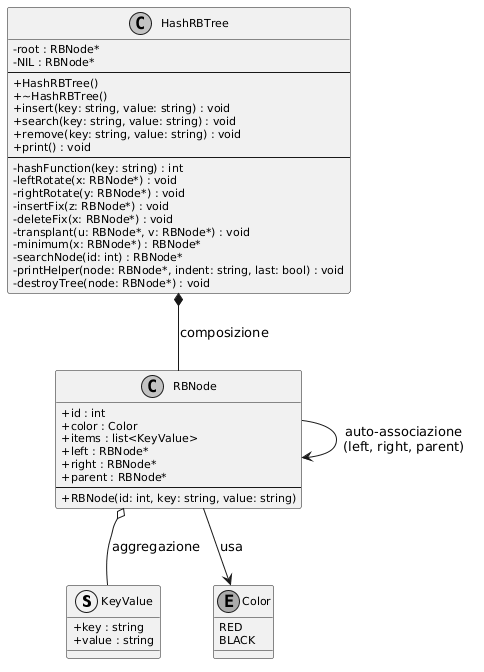
\includegraphics[width=\textwidth]{images/classdiagram.png}
\caption{Class diagram UML di HashRBTree}
\label{fig:classdiagram}
\end{figure}

\section{Relazioni tra le Classi}

\begin{itemize}
    \item \textbf{HashRBTree} ha una relazione di \textbf{composizione} con 
    \texttt{RBNode}: i nodi sono creati e distrutti esclusivamente dalla classe 
    \texttt{HashRBTree} tramite i metodi \texttt{insert} e \texttt{destroyTree}.
    \item \textbf{RBNode} ha una relazione di \textbf{aggregazione} con 
    \texttt{KeyValue}: ogni nodo contiene una \texttt{std::list<KeyValue>} 
    che può ospitare una o più coppie chiave-valore in caso di collisione.
    \item \textbf{RBNode} ha una relazione di \textbf{auto-associazione} 
    tramite i puntatori \texttt{left}, \texttt{right} e \texttt{parent}, 
    che collegano i nodi tra loro formando la struttura ad albero.
    \item Il tipo enumerato \textbf{Color} (\texttt{RED}, \texttt{BLACK}) 
    è utilizzato da \texttt{RBNode} per mantenere le proprietà cromatiche 
    del Red-Black Tree.
\end{itemize}
\chapter{Studio della Complessità}

In questo capitolo viene analizzata la complessità temporale e spaziale 
delle operazioni principali della struttura \texttt{HashRBTree}.

\section{Complessità Temporale}

\subsection{Funzione di Hash}

La funzione \texttt{hashFunction} itera su tutti i caratteri della chiave 
eseguendo un numero costante di operazioni per ciascuno. La complessità è:

\begin{equation}
    T_{hash} = O(m)
\end{equation}

dove $m$ è la lunghezza della chiave in caratteri.

\subsection{Ricerca nell'Albero}

Il metodo \texttt{searchNode} naviga l'albero Red-Black dall'alto verso il 
basso confrontando il valore \texttt{id} ad ogni nodo. Poiché l'albero è 
bilanciato per costruzione, l'altezza è garantita essere $O(\log n)$, dove 
$n$ è il numero di nodi distinti nell'albero. La complessità è:

\begin{equation}
    T_{searchNode} = O(\log n)
\end{equation}

\subsection{Ricerca nella Lista di Collisione}

Una volta individuato il nodo tramite \texttt{searchNode}, il metodo 
\texttt{search} scorre la lista \texttt{items} per trovare la chiave esatta. 
Indicando con $k$ il numero di coppie in collisione su quel nodo:

\begin{equation}
    T_{search} = O(m + \log n + k)
\end{equation}

Nel caso medio, con una buona funzione di hash, $k$ è costante e la 
complessità si riduce a $O(m + \log n)$.

\subsection{Inserimento}

L'operazione \texttt{insert} esegue in sequenza:

\begin{enumerate}
    \item Calcolo dell'hash: $O(m)$
    \item Ricerca del nodo: $O(\log n)$
    \item In caso di collisione, aggiunta in coda alla lista: $O(k)$
    \item In caso di nuovo nodo, inserimento BST: $O(\log n)$
    \item Ripristino proprietà RBT con \texttt{insertFix}: $O(\log n)$
\end{enumerate}

La complessità complessiva è:

\begin{equation}
    T_{insert} = O(m + \log n)
\end{equation}

\texttt{insertFix} esegue al più $O(\log n)$ recoloring risalendo l'albero, 
e al più 2 rotazioni che sono operazioni $O(1)$.

\subsection{Cancellazione}

L'operazione \texttt{remove} esegue in sequenza:

\begin{enumerate}
    \item Calcolo dell'hash: $O(m)$
    \item Ricerca del nodo: $O(\log n)$
    \item Rimozione dalla lista: $O(k)$
    \item Se la lista è vuota, rimozione dall'albero: $O(\log n)$
    \item Ripristino proprietà RBT con \texttt{deleteFix}: $O(\log n)$
\end{enumerate}

La complessità complessiva è:

\begin{equation}
    T_{remove} = O(m + \log n)
\end{equation}

\texttt{deleteFix} esegue al più $O(\log n)$ recoloring e al più 3 rotazioni.

\subsection{Riepilogo}

\begin{center}
\begin{tabular}{|l|c|c|}
\hline
\textbf{Operazione} & \textbf{Caso Medio} & \textbf{Caso Peggiore} \\
\hline
\texttt{hashFunction} & $O(m)$ & $O(m)$ \\
\hline
\texttt{search}       & $O(m + \log n)$ & $O(m + \log n + k)$ \\
\hline
\texttt{insert}       & $O(m + \log n)$ & $O(m + \log n + k)$ \\
\hline
\texttt{remove}       & $O(m + \log n)$ & $O(m + \log n + k)$ \\
\hline
\end{tabular}
\end{center}

\vspace{0.5cm}
dove $n$ è il numero di nodi nell'albero, $m$ è la lunghezza della chiave 
e $k$ è il numero di collisioni sul nodo.

\section{Complessità Spaziale}

La struttura occupa in memoria:

\begin{itemize}
    \item $O(n)$ per i nodi dell'albero, dove $n$ è il numero di chiavi 
    distinte per hash;
    \item $O(n + p)$ considerando anche le coppie nelle liste di collisione, 
    dove $p$ è il numero totale di coppie inserite;
    \item $O(\log n)$ per lo stack delle chiamate ricorsive di 
    \texttt{printHelper} e \texttt{destroyTree}.
\end{itemize}

La complessità spaziale complessiva è:

\begin{equation}
    S = O(n + p)
\end{equation}
\chapter{Test e Risultati}

In questo capitolo vengono presentati i test eseguiti sulla struttura 
\texttt{HashRBTree} per verificare la correttezza delle operazioni di 
inserimento, ricerca, cancellazione e stampa.

\section{Ambiente di Test}

I test sono stati eseguiti nel seguente ambiente:

\begin{itemize}
    \item \textbf{Sistema operativo}: Linux Mint
    \item \textbf{Compilatore}: GCC 13.3.0
    \item \textbf{Standard}: C++17
    \item \textbf{Build system}: CMake 3.10
\end{itemize}

\section{Test 1 --- Inserimento e Stampa}

Vengono inserite sette coppie chiave-valore e viene verificata la struttura 
dell'albero tramite \texttt{print()}.

\begin{lstlisting}
tree.insert("apple",      "frutto rosso");
tree.insert("banana",     "frutto giallo");
tree.insert("cherry",     "frutto rosso piccolo");
tree.insert("date",       "frutto dolce");
tree.insert("elderberry", "frutto viola");
tree.insert("fig",        "frutto mediterraneo");
tree.insert("grape",      "frutto a grappolo");
\end{lstlisting}

\textbf{Output ottenuto}:

\begin{lstlisting}
+-- [1938937894 | B] banana:frutto giallo
    +-- [253337143 | R] apple:frutto rosso
    |   +-- [193491643 | B] fig:frutto mediterraneo
    |   `-- [735886645 | B] elderberry:frutto viola
    |       +-- [260508340 | R] grape:frutto a grappolo
    `-- [1986069970 | B] cherry:frutto rosso piccolo
        `-- [2090176867 | R] date:frutto dolce
\end{lstlisting}

\textbf{Verifica}: l'albero rispetta tutte le proprietà del Red-Black Tree:
\begin{itemize}
    \item la radice è \texttt{BLACK};
    \item non esistono due nodi \texttt{RED} consecutivi;
    \item il black-height è uniforme su tutti i percorsi dalla radice 
    alle foglie.
\end{itemize}

\section{Test 2 --- Ricerca}

\begin{lstlisting}
tree.search("apple",  "");
tree.search("banana", "");
tree.search("mango",  "");
\end{lstlisting}

\textbf{Output ottenuto}:

\begin{lstlisting}
Trovato: apple -> frutto rosso
Trovato: banana -> frutto giallo
Chiave "mango" non trovata.
\end{lstlisting}

\textbf{Verifica}: le chiavi presenti vengono trovate correttamente; 
la ricerca di una chiave assente restituisce il messaggio di errore 
senza crash.

\section{Test 3 --- Gestione delle Collisioni}

Vengono inserite due chiavi aggiuntive per verificare il comportamento 
in caso di collisioni hash.

\begin{lstlisting}
tree.insert("listen", "ascoltare");
tree.insert("silent", "silenzioso");
\end{lstlisting}

\textbf{Verifica}: la funzione djb2 è sensibile all'ordine dei caratteri, 
quindi \texttt{listen} e \texttt{silent} producono hash distinti e vengono 
inseriti come nodi separati. L'albero si ribilancia correttamente dopo 
entrambi gli inserimenti.

\section{Test 4 --- Cancellazione}

\begin{lstlisting}
tree.remove("banana", "");
tree.remove("mango",  "");
\end{lstlisting}

\textbf{Output ottenuto}:

\begin{lstlisting}
Chiave "mango" non trovata.

+-- [1986069970 | B] cherry:frutto rosso piccolo
    +-- [253337143 | R] apple:frutto rosso
    |   +-- [193491643 | B] fig:frutto mediterraneo
    |   |   +-- [192495636 | R] listen:ascoltare
    |   `-- [466175796 | B] silent:silenzioso
    |       +-- [260508340 | R] grape:frutto a grappolo
    |       `-- [735886645 | R] elderberry:frutto viola
    `-- [2090176867 | B] date:frutto dolce
\end{lstlisting}

\textbf{Verifica}: la rimozione di \texttt{banana} (nodo radice) viene 
gestita correttamente tramite il successore in-order; l'albero rimane 
bilanciato. La rimozione di \texttt{mango} (chiave assente) produce 
il messaggio di errore senza alterare la struttura.

\section{Test 5 --- Cancellazioni Multiple}

\begin{lstlisting}
tree.remove("apple",  "");
tree.remove("cherry", "");
\end{lstlisting}

\textbf{Output ottenuto}:

\begin{lstlisting}
+-- [260508340 | B] grape:frutto a grappolo
    +-- [193491643 | B] fig:frutto mediterraneo
    |   +-- [192495636 | R] listen:ascoltare
    `-- [735886645 | R] elderberry:frutto viola
        +-- [466175796 | B] silent:silenzioso
        `-- [2090176867 | B] date:frutto dolce
\end{lstlisting}

\textbf{Verifica}: dopo tre cancellazioni consecutive l'albero rimane 
correttamente bilanciato, confermando il corretto funzionamento di 
\texttt{deleteFix} in scenari di stress.

\section{Considerazioni Finali}

I test confermano che la struttura \texttt{HashRBTree} si comporta 
correttamente in tutti gli scenari verificati:

\begin{itemize}
    \item le proprietà del Red-Black Tree vengono mantenute dopo ogni 
    inserimento e cancellazione;
    \item la gestione delle collisioni tramite lista funziona correttamente;
    \item i casi limite (chiave assente, albero con un solo nodo, 
    cancellazione della radice) sono gestiti senza errori.
\end{itemize}

\end{document}